\documentclass{beamer}
\usetheme{Berlin}
\usepackage[T1]{fontenc}
\usepackage{minted}
\usepackage{etoolbox}
\usepackage{setspace}
\usepackage{bussproofs}
\usepackage{amsmath}
\usepackage{amsthm}
\usepackage{amssymb}
\usepackage{amsxtra}
\usepackage{csquotes}
\usepackage{tcolorbox}
\usepackage{booktabs}
\usepackage[croatian]{babel}
\usepackage{forest}
\graphicspath{{./img}}

\newcommand\coqset{\texttt{Set}}
\newcommand\coqprop{\texttt{Prop}}
\newcommand\coqtype[1]{\texttt{Type\(_{#1}\)}}
\DeclareRobustCommand{\VDash}{\mathrel{||}\joinrel\Relbar}

\BeforeBeginEnvironment{minted}{\begin{spacing}{1.0}\begin{tcolorbox}}
    \AfterEndEnvironment{minted}{\end{tcolorbox}\end{spacing}}

\DeclareUnicodeCharacter{22A8}{\(\vDash\)}
\DeclareUnicodeCharacter{22A2}{\(\vdash\)}
\DeclareUnicodeCharacter{2286}{\(\subseteq\)}
\DeclareUnicodeCharacter{22AB}{\(\VDash\)}
\DeclareUnicodeCharacter{2291}{\(\sqsubseteq\)}
\DeclareUnicodeCharacter{03A3}{\(\Sigma\)}
\DeclareUnicodeCharacter{03C1}{\(\rho\)}
\DeclareUnicodeCharacter{03C6}{\(\varphi\)}
\DeclareUnicodeCharacter{03A6}{\(\Phi\)}
\DeclareUnicodeCharacter{03B1}{\(\alpha\)}
\DeclareUnicodeCharacter{03C9}{\(\omega\)}
\DeclareUnicodeCharacter{0393}{\(\Gamma\)}
\DeclareUnicodeCharacter{0394}{\(\Delta\)}
\DeclareUnicodeCharacter{03C8}{\(\psi\)}
\DeclareUnicodeCharacter{03C3}{\(\sigma\)}
\DeclareUnicodeCharacter{03BA}{\(\kappa\)}
\DeclareUnicodeCharacter{03B2}{\(\beta\)}
\title{Primjene Coq alata za dokazivanje u matematici i računarstvu}
\subtitle{Logika prvog reda s induktivnim definicijama}
\author{Miho Hren}
\institute{Mentori: Vedran Čačić, Marko Doko \(+\) Ante Đerek\\
  Fakultet Elektrotehnike i Računarstva}
\date{2023./2024.}

\setbeamertemplate{headline}{}
\setbeamertemplate{footline}[frame number]
\setbeamertemplate{navigation symbols}{}


\begin{document}
\begin{frame}
  \titlepage{}
\end{frame}

\begin{frame}
  \frametitle{Što je Coq?}
  \begin{itemize}
  \item programski jezik
  \item \textbf{interaktivni dokazivač teorema} --- stroj provjerava dokaz
  \item temeljen na teoriji tipova
  \end{itemize}
  \begin{align*}
    \mathit{propozicija} & = \mathit{tip} \\
    \mathit{dokaz} & = \mathit{program}
  \end{align*}
  \begin{itemize}
  \item u matematici: \textbf{teorem o četiri boje}, temelji matematike, \textit{obrazovanje}
  \item u računarstvu: \textbf{CompCert}, VeLLVM, CertiKOS, certificirano programiranje
  \end{itemize}

  \begin{alertblock}{Zašto?}
    \centering
    Kritična infrastruktura!
  \end{alertblock}  
\end{frame}

\begin{frame}[plain]
  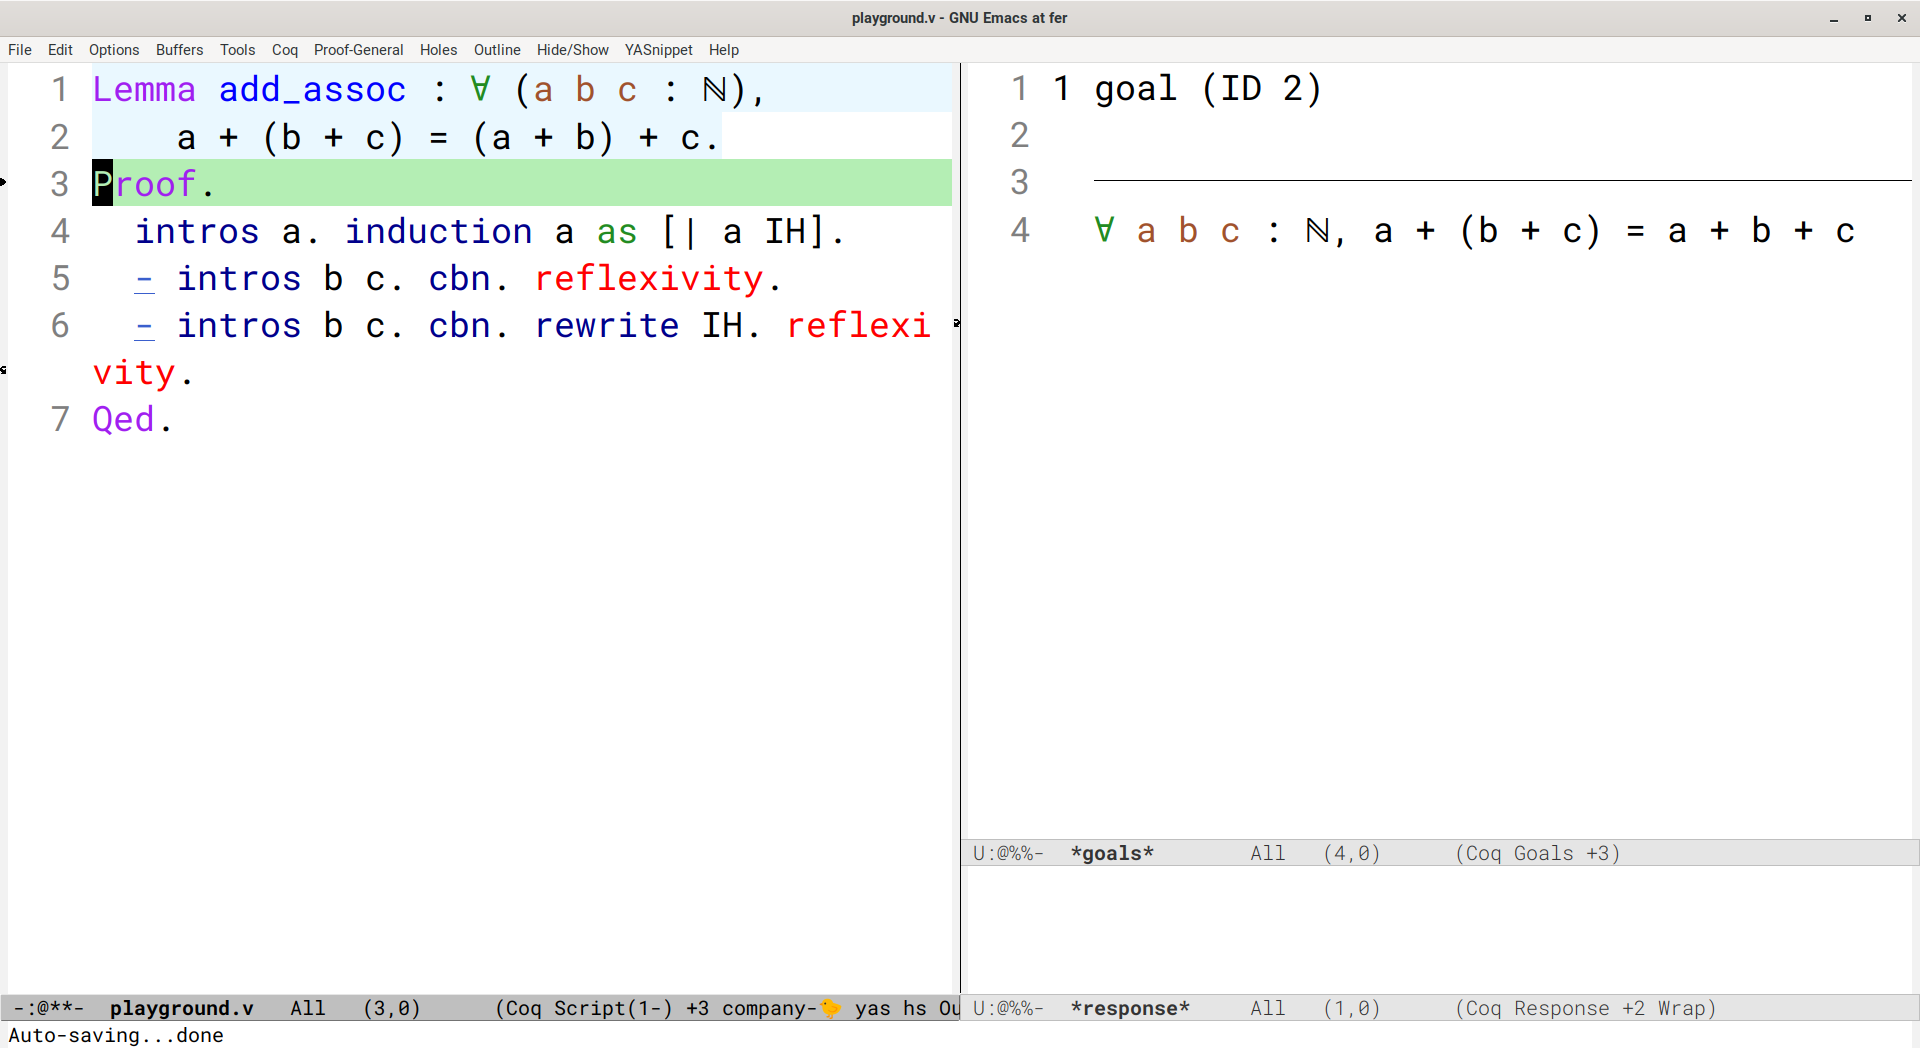
\includegraphics[width=\linewidth]{slika1}
\end{frame}\addtocounter{framenumber}{-1}
\begin{frame}[plain]
  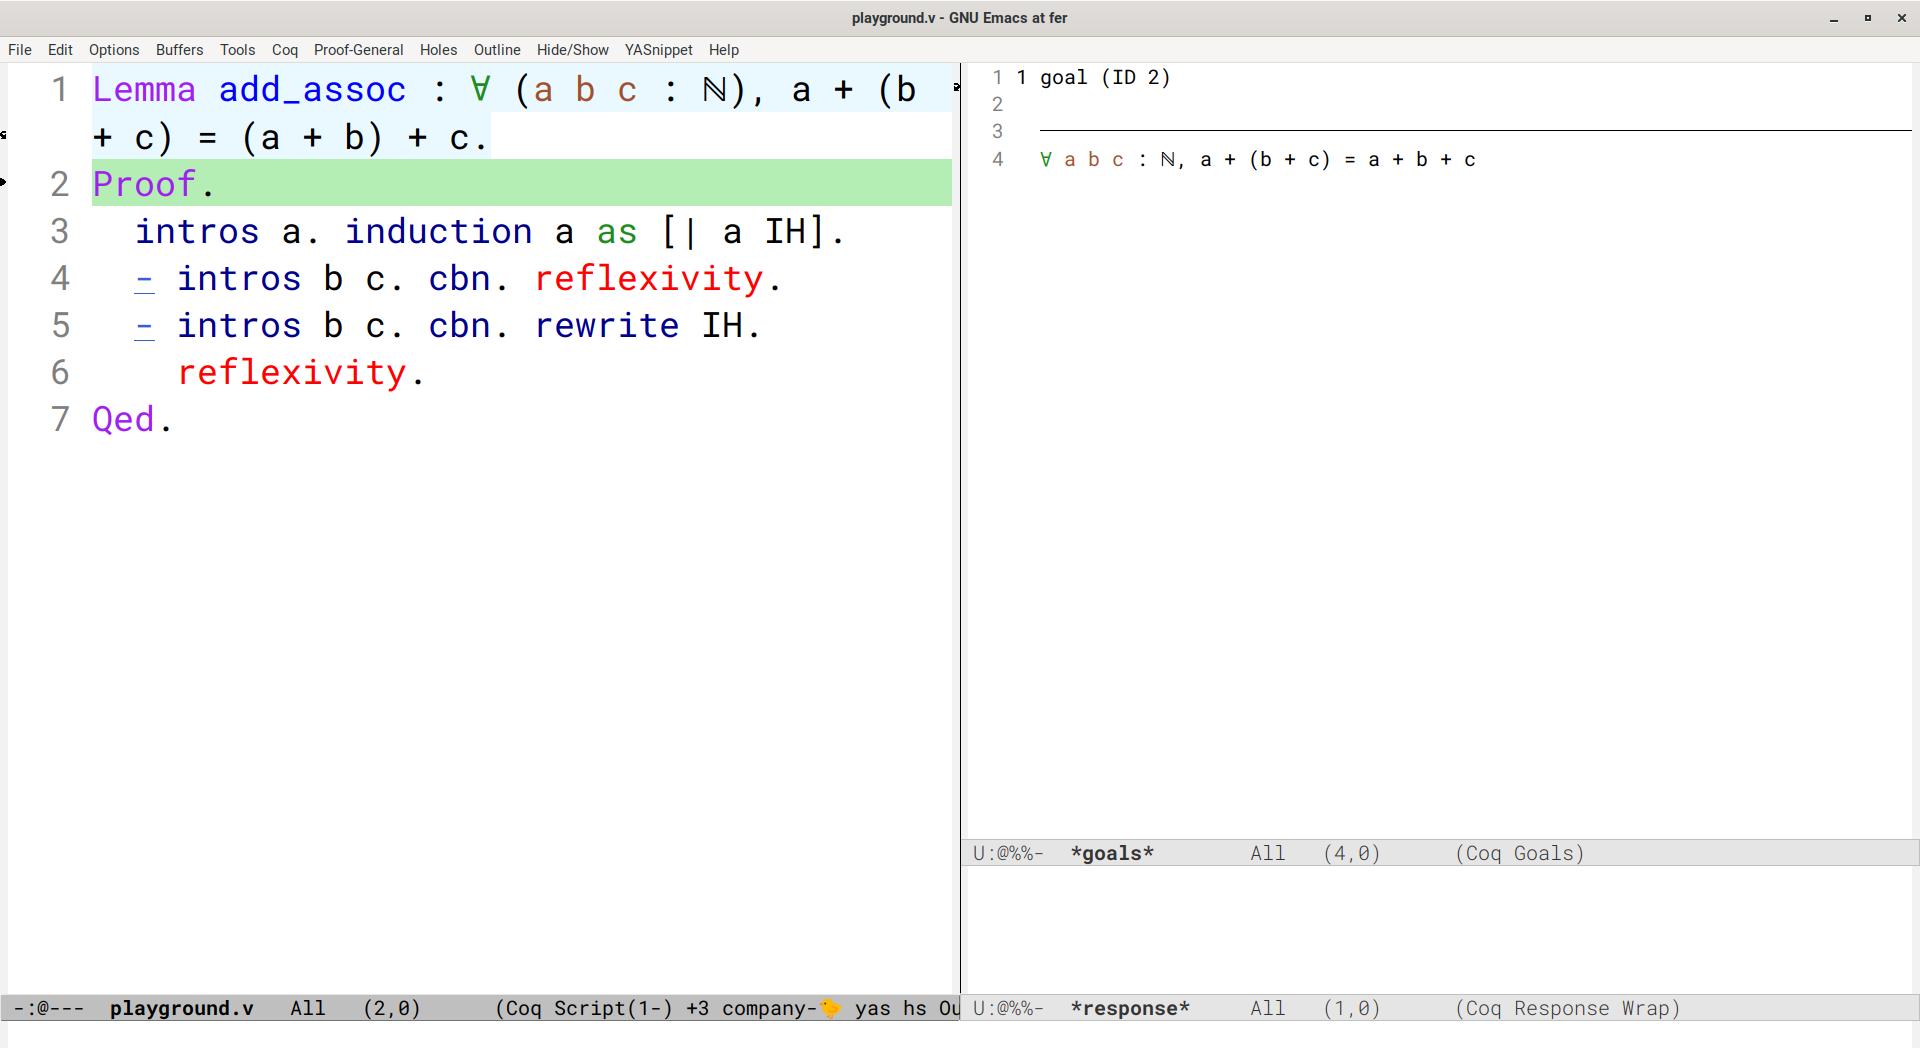
\includegraphics[width=\linewidth]{slika3}
\end{frame}\addtocounter{framenumber}{-1}
\begin{frame}[plain]
  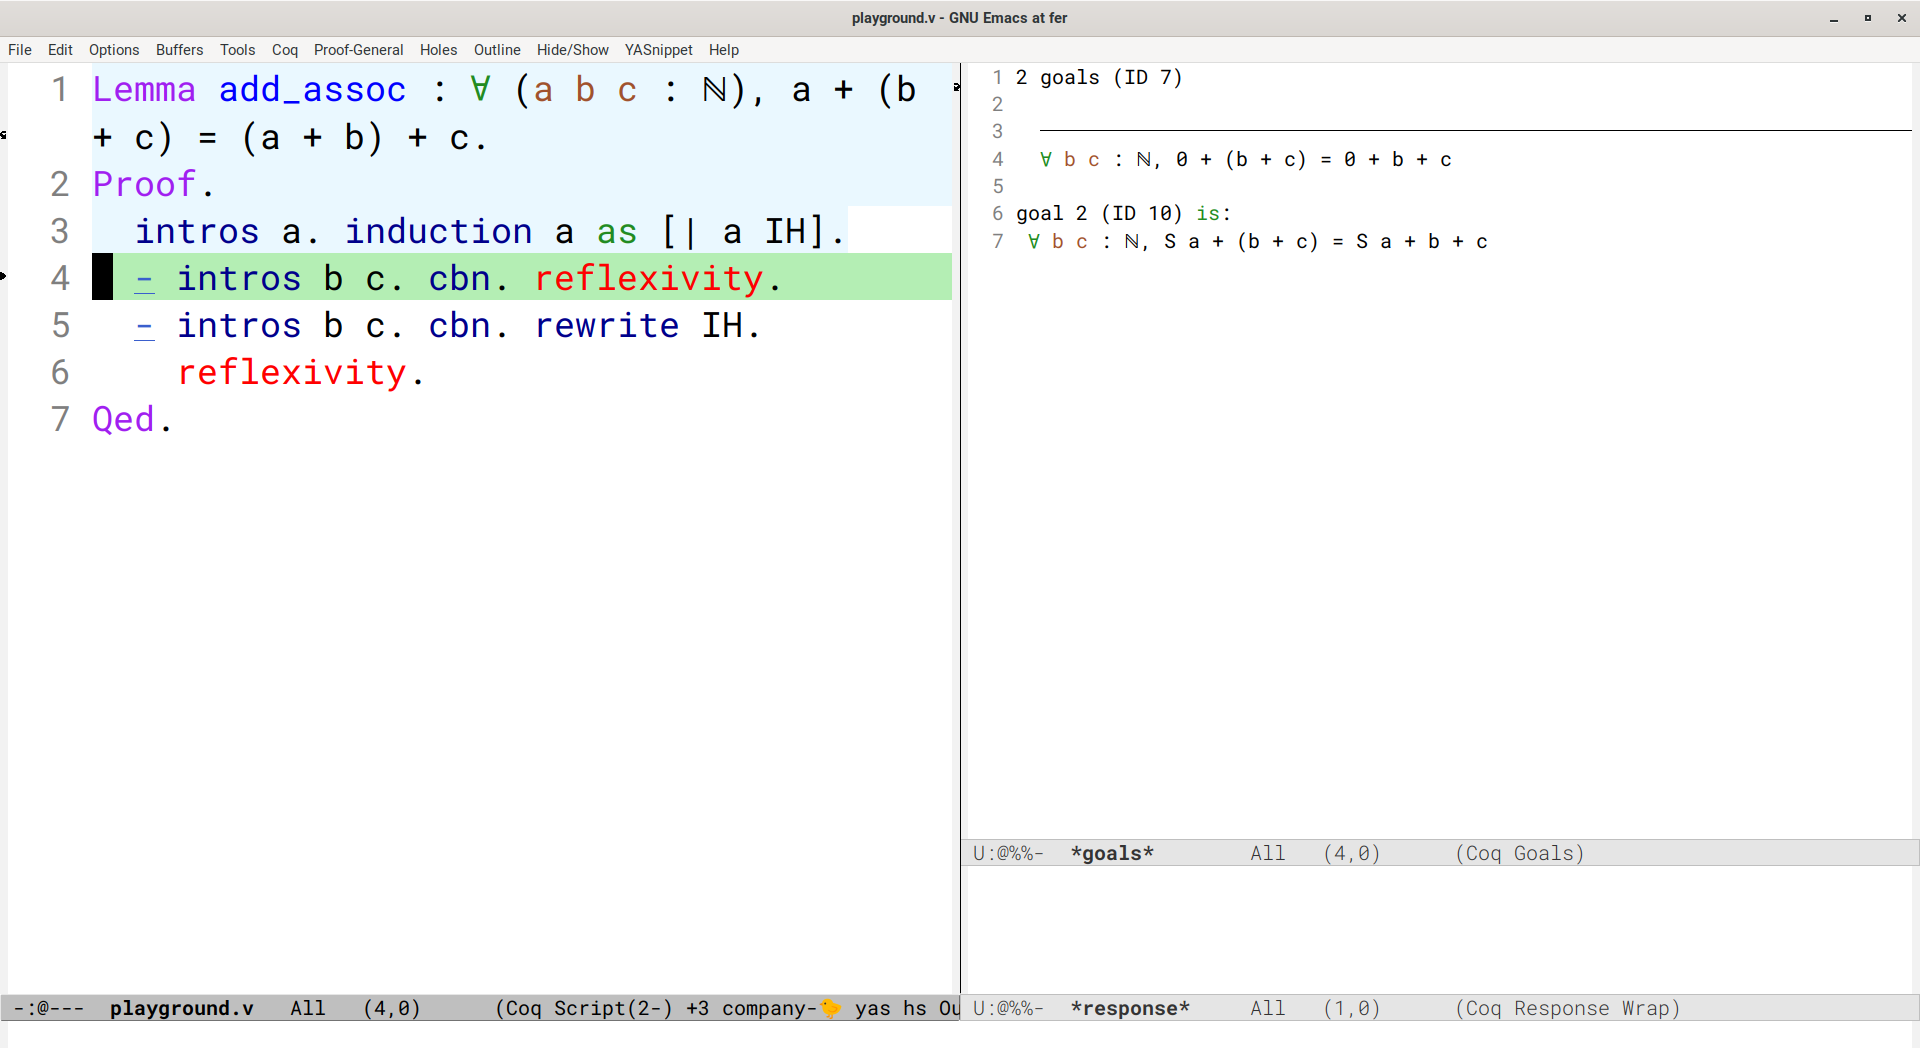
\includegraphics[width=\linewidth]{slika5}
\end{frame}\addtocounter{framenumber}{-1}
\begin{frame}[plain]
  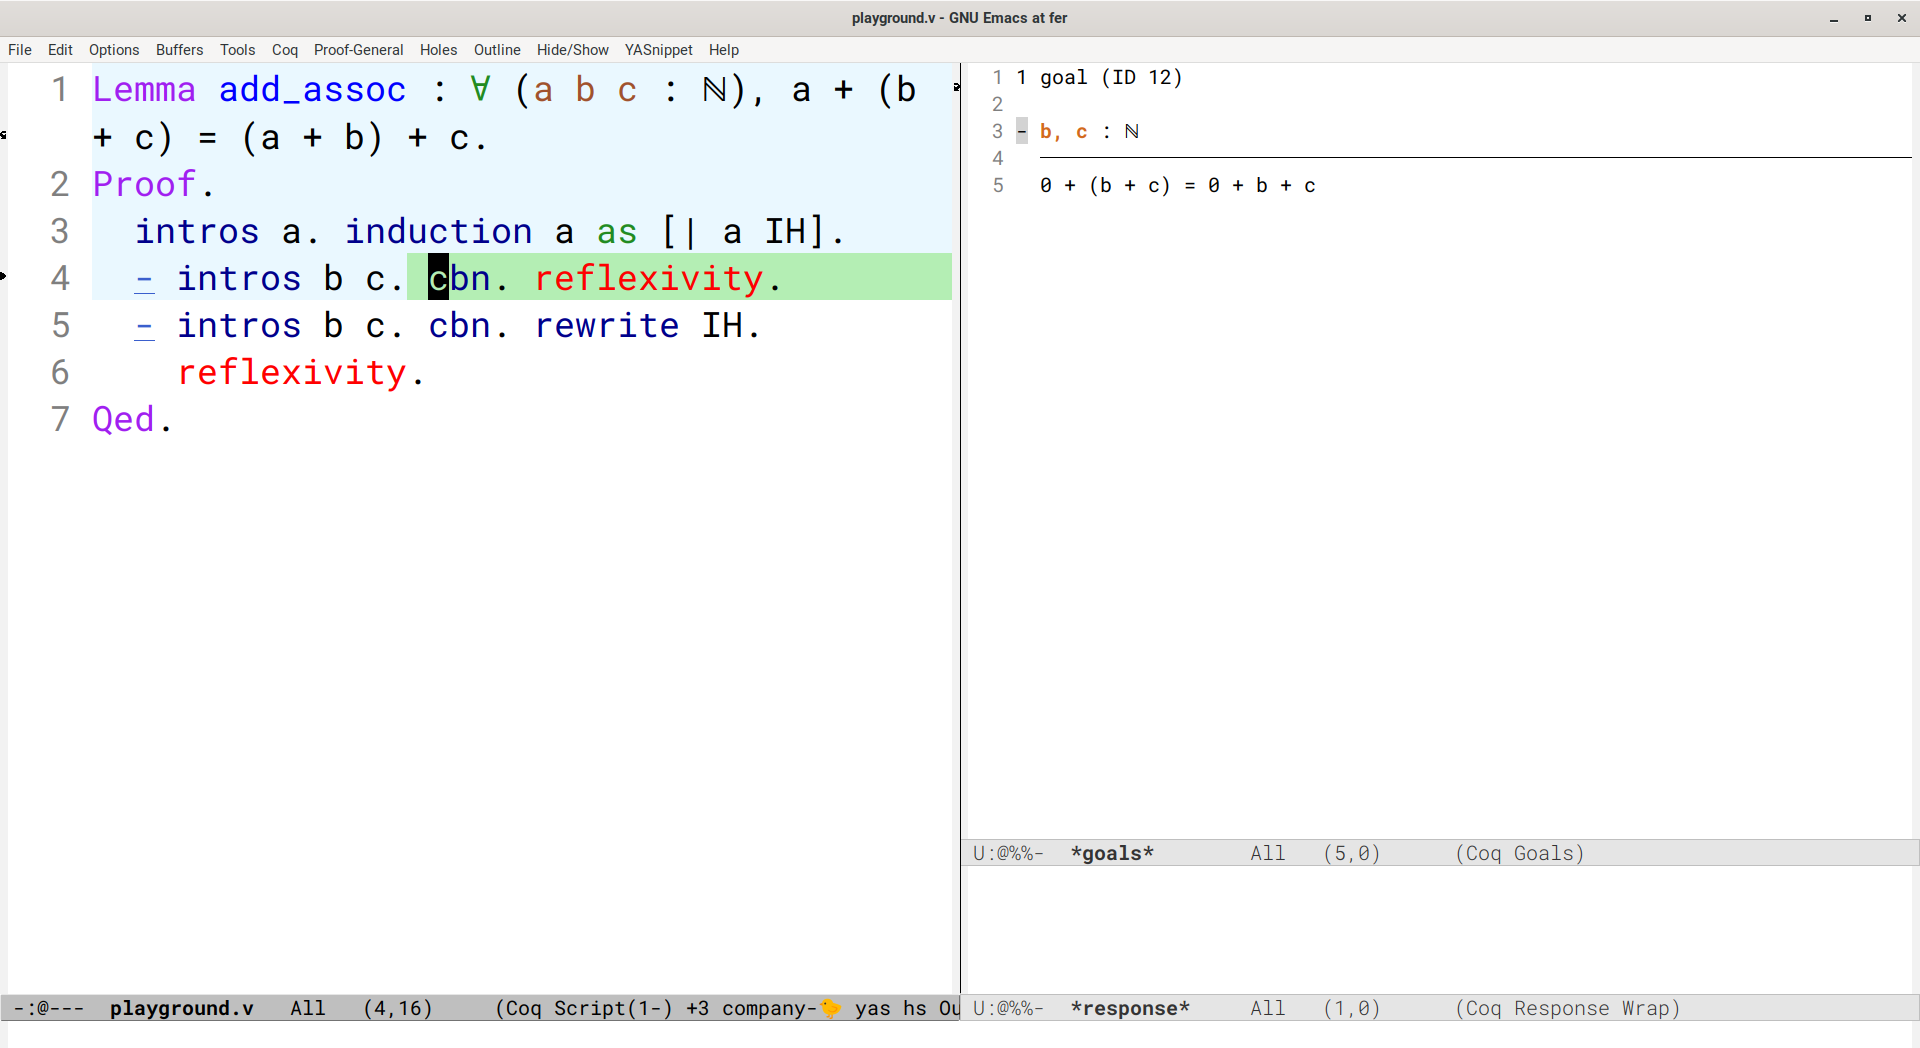
\includegraphics[width=\linewidth]{slika7}
\end{frame}\addtocounter{framenumber}{-1}
\begin{frame}[plain]
  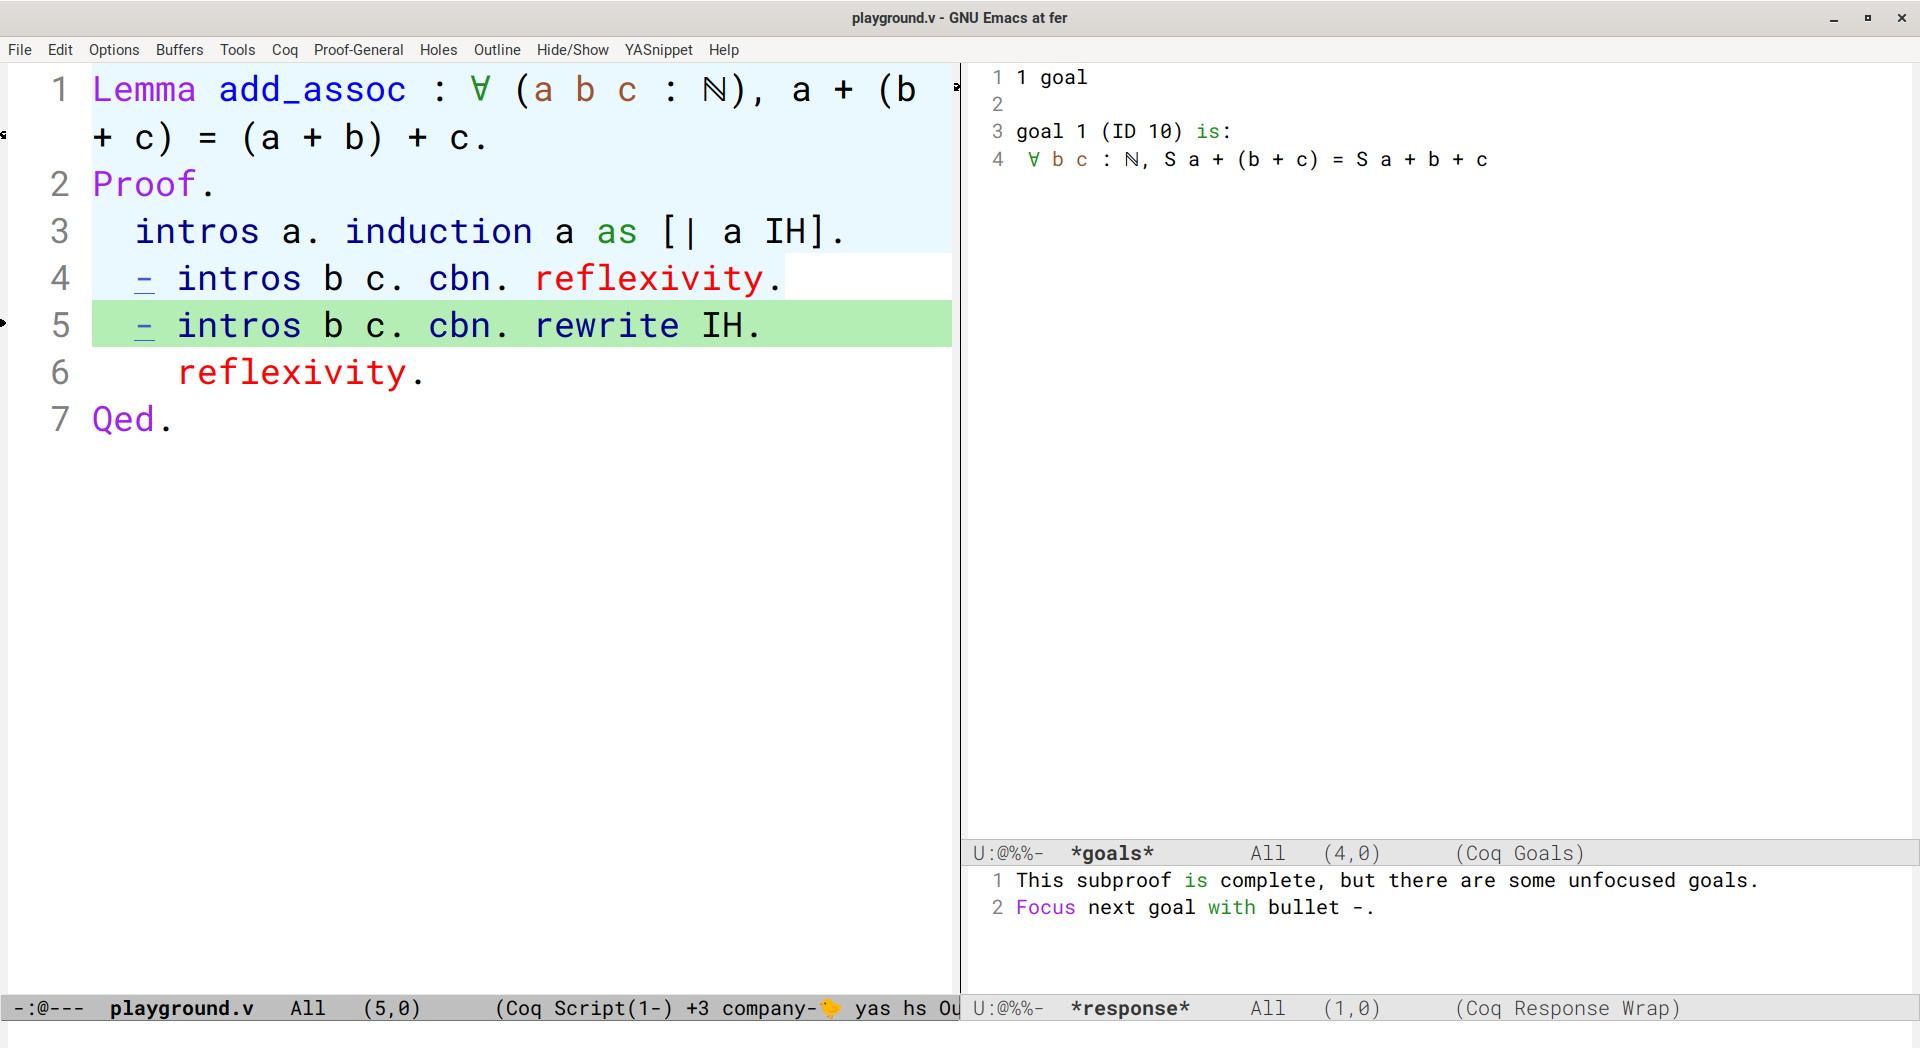
\includegraphics[width=\linewidth]{slika9}
\end{frame}\addtocounter{framenumber}{-1}
\begin{frame}[plain]
  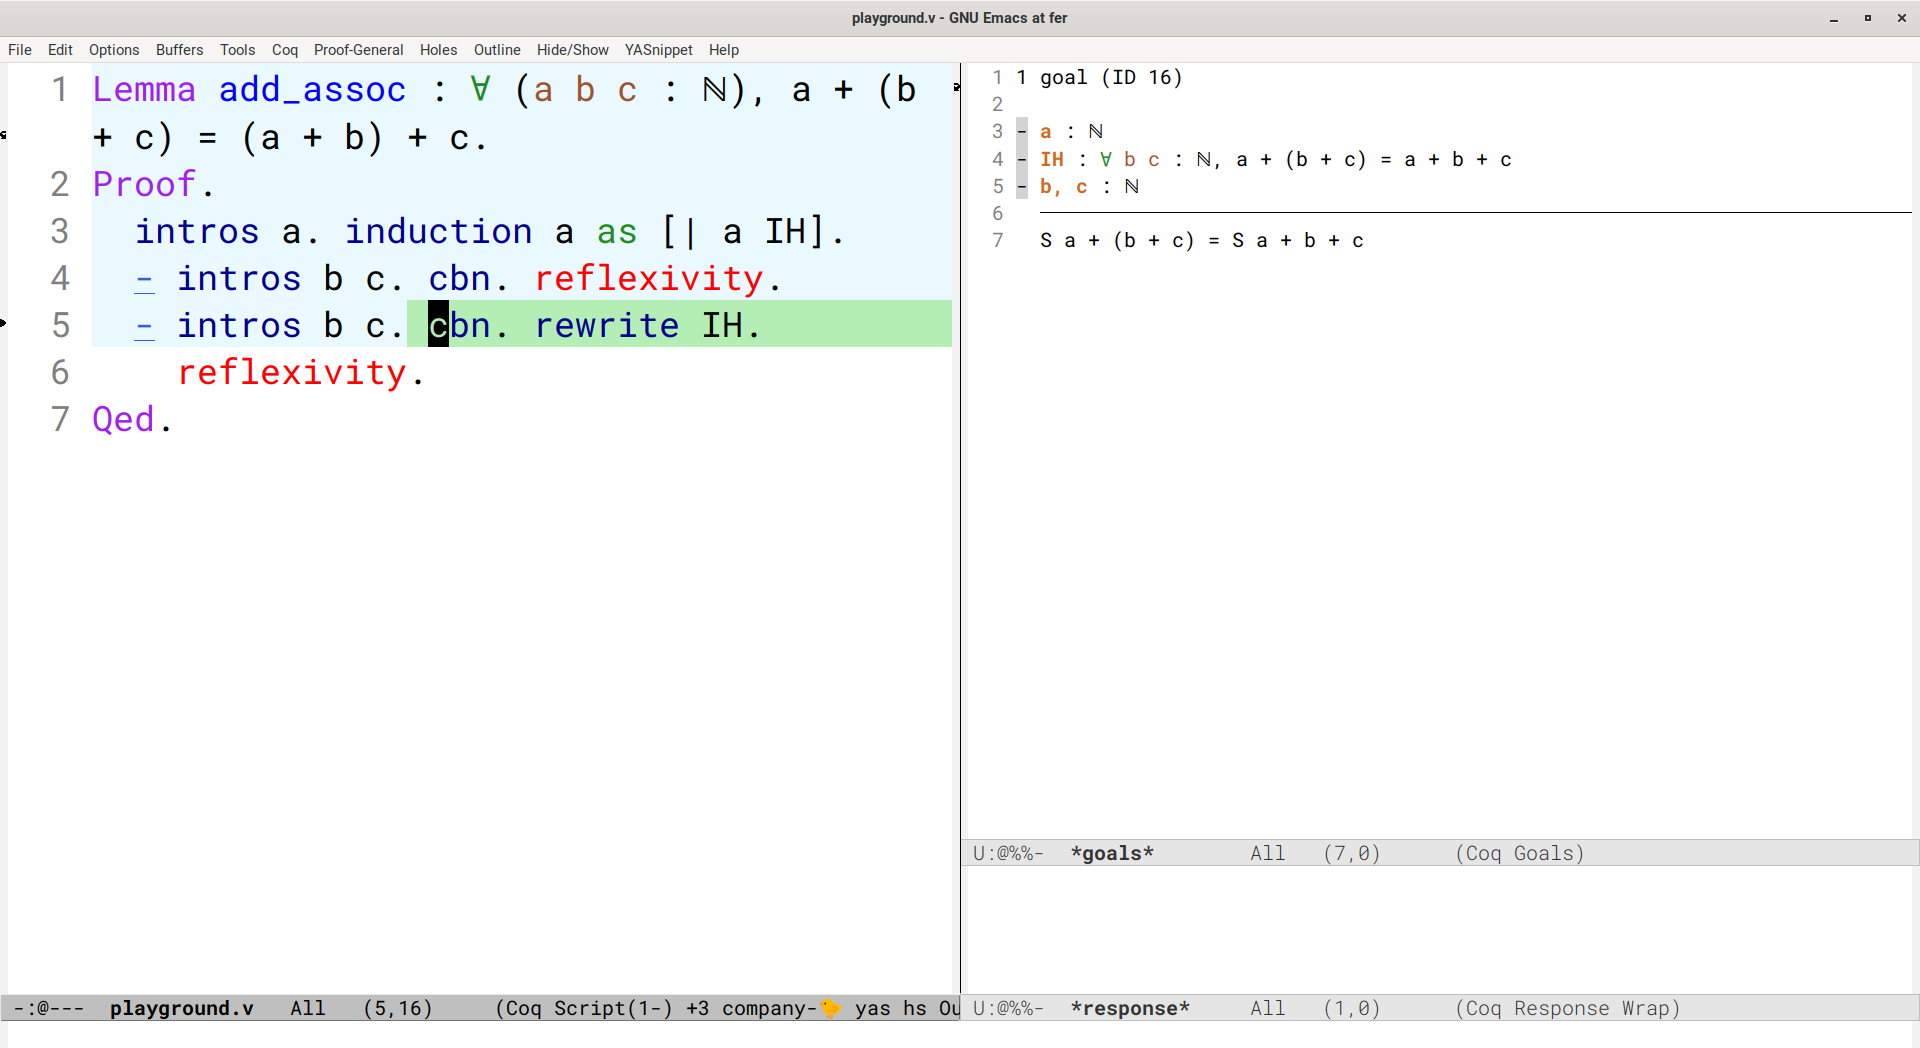
\includegraphics[width=\linewidth]{slika11}
\end{frame}\addtocounter{framenumber}{-1}
\begin{frame}[plain]
  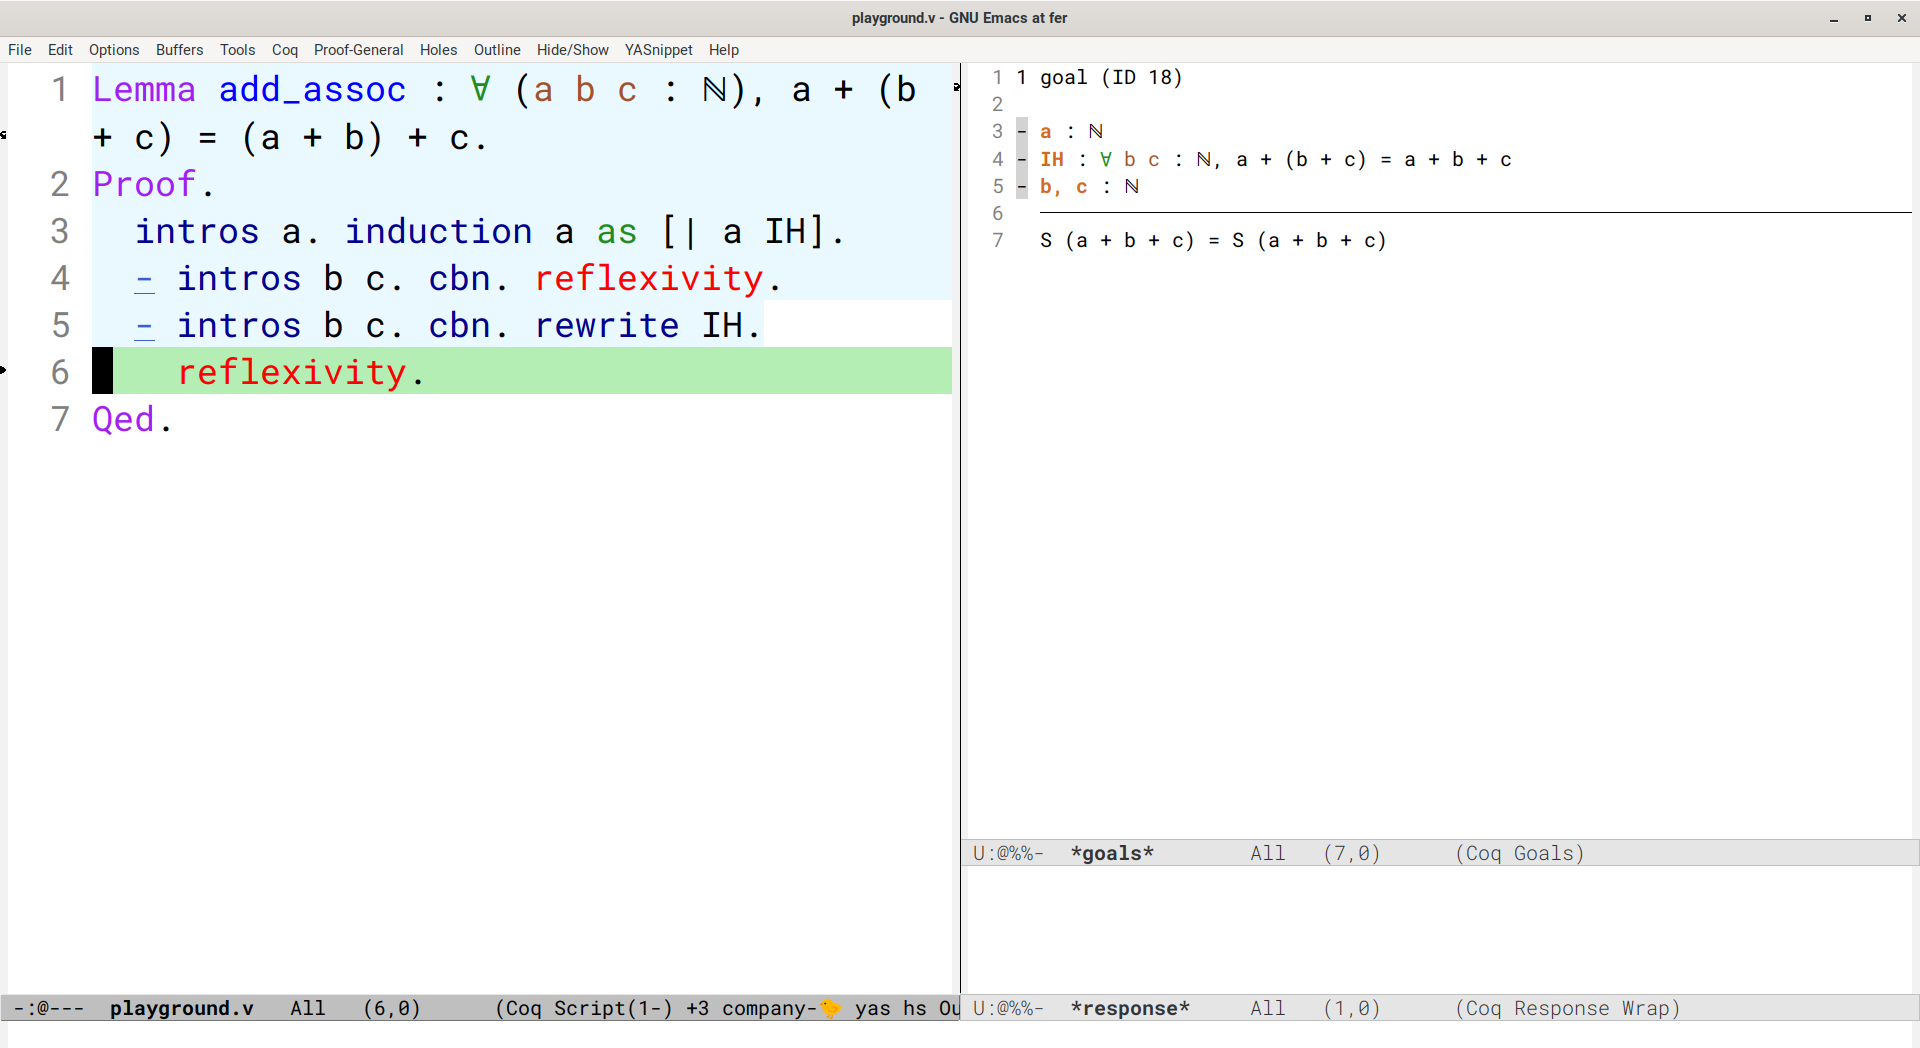
\includegraphics[width=\linewidth]{slika13}
\end{frame}\addtocounter{framenumber}{-1}
\begin{frame}[plain]
  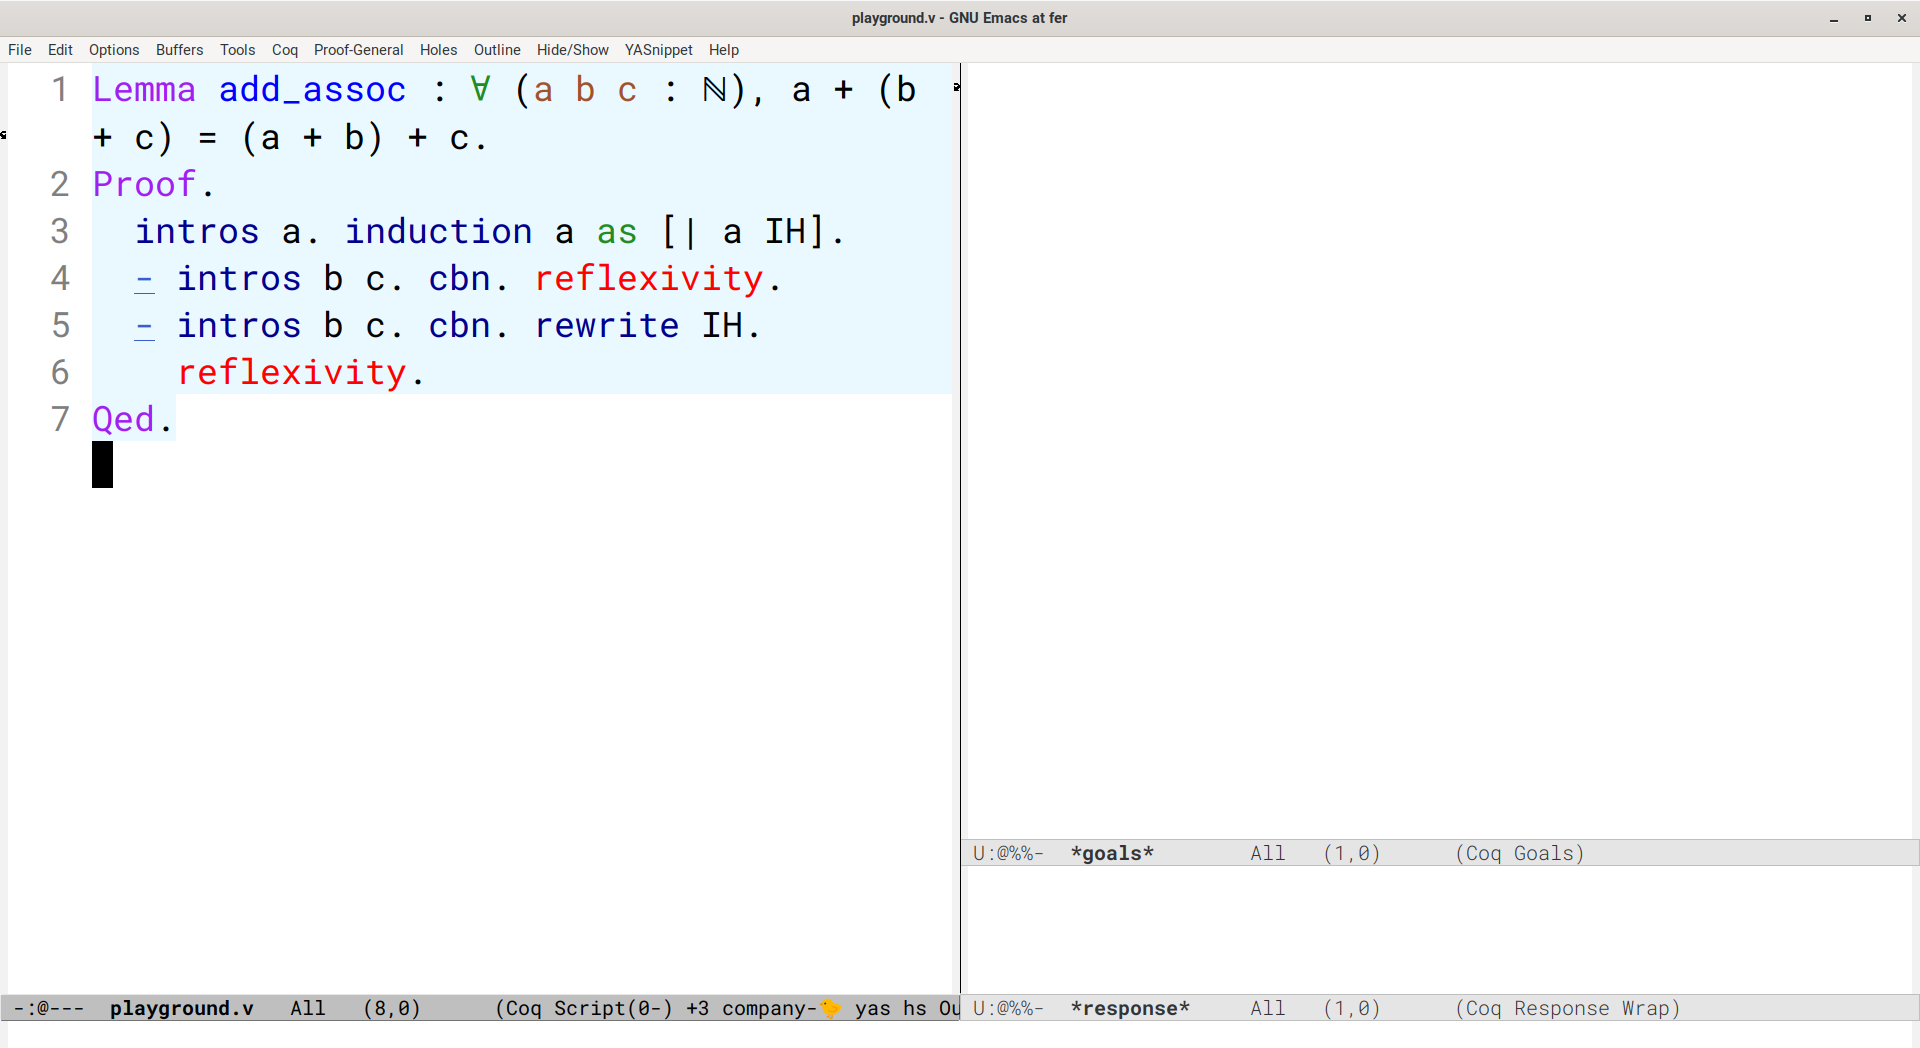
\includegraphics[width=\linewidth]{slika15}
\end{frame}\addtocounter{framenumber}{-1}

  
\begin{frame}
  \frametitle{Proces}
  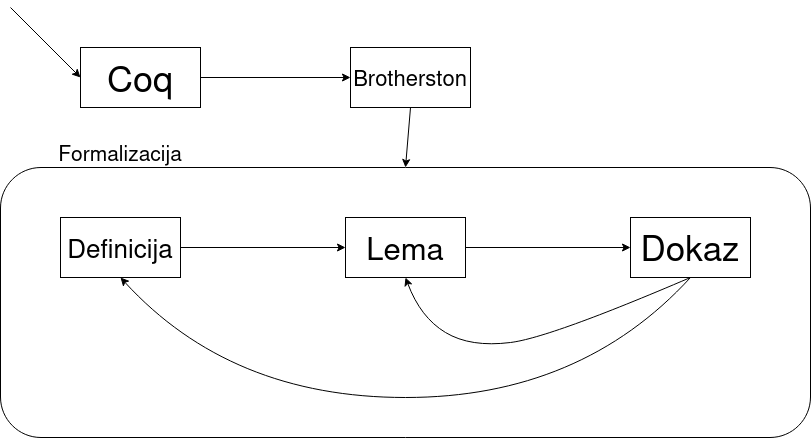
\includegraphics[width=\textwidth]{diplomskiproces.png}
\end{frame}

\begin{frame}[fragile]
  \frametitle{Sintaksa: signatura}
  \begin{center}
    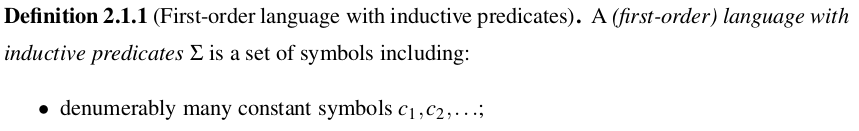
\includegraphics[width=0.6\linewidth]{signatura1}
    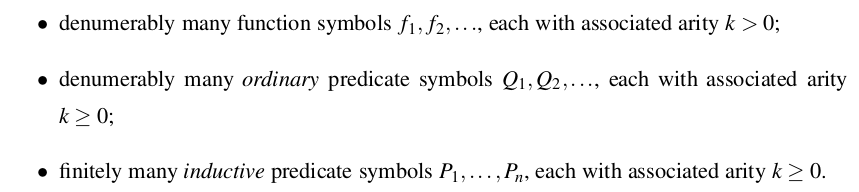
\includegraphics[width=0.6\linewidth]{signatura2}
  \end{center}
  \begin{scriptsize}
\begin{minted}{coq}
Structure signature := {
    FuncS : Set;
    fun_ar : FuncS -> nat;
    PredS : Set;
    pred_ar : PredS -> nat;
    IndPredS : Set;
    indpred_ar : IndPredS -> nat;
  }.
\end{minted}
  \end{scriptsize}
  \begin{block}{Primjer: Peanova signatura}
      \[
    \sigma_{\mathit{PA}} = \{ \{ o^{0}, s^{1}, +^{2}, \cdot^{2} \},
    \{=^{2}\}, \{\mathit{Nat}^{1}, \mathit{Even}^{1}, \mathit{Odd}^{1}\}\}
  \]
  \end{block}
\end{frame}

\begin{frame}[fragile,fragile,fragile]{Sintaksa: termi}
  \begin{center}
    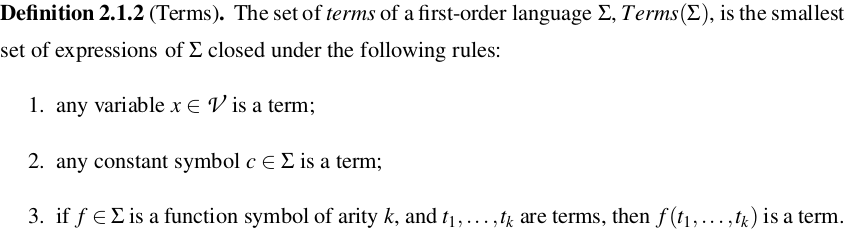
\includegraphics[width=0.6\linewidth]{term}
  \end{center}
  \begin{footnotesize}
\begin{minted}{coq}
Inductive term  : Set :=
| var_term : var -> term 
| TFunc : forall (f : FuncS Σ),
    vec term (fun_ar f) -> term.
\end{minted}
  \end{footnotesize}
  \begin{block}{Primjeri terma}
    \[
      s(o), s(s(x)), f(x, v, w, g(z, q))
    \]
  \end{block}
  \begin{footnotesize}
\begin{minted}{coq}
Example PA_one (* s(o) *): term Σ__PA :=
  TFunc PA_succ [TFunc PA_zero []].
\end{minted}
  \end{footnotesize}
\end{frame}


\begin{frame}[fragile]
  \frametitle{Sintaksa: formula}
  \begin{center}
    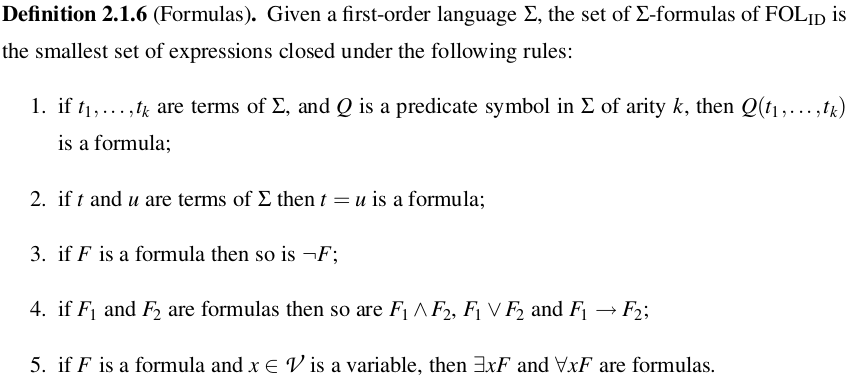
\includegraphics[width=0.6\linewidth]{formula}
  \end{center}
\begin{minted}{coq}
Inductive formula : Set :=
| FPred (P : PredS Σ)
    : vec (term Σ) (pred_ar P) -> formula 
| FIndPred (P : IndPredS Σ)
    : vec (term Σ) (indpred_ar P) -> formula 
| FNeg : formula -> formula 
| FImp : formula -> formula -> formula 
| FAll : formula -> formula.
\end{minted}
\end{frame}

\begin{frame}[fragile]
  \frametitle{Sintaksa: formula}
  \begin{block}{Primjer formule}
    \[
      \forall x, \mathit{Nat}(x) \rightarrow \mathit{Even}(x) \lor \mathit{Odd}(x)
    \]
  \end{block}
\begin{minted}{coq}
Definition every_nat_is_even_or_odd
  : formula Σ__PA :=
  let x := var_term 0 in
  FAll
    (FImp
       (FIndPred PA_Nat [x])
       (FOr
          (FIndPred PA_Even [x])
          (FIndPred PA_Odd  [x]))).
\end{minted}
\end{frame}

\begin{frame}[fragile]
  \frametitle{Sintaksa: produkcije}
  \begin{center}
    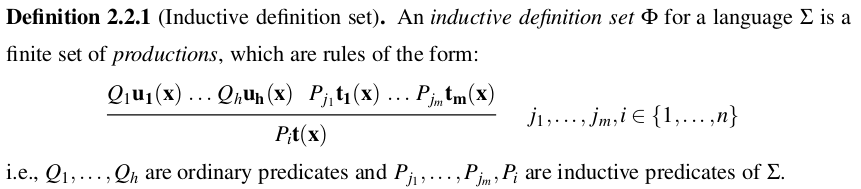
\includegraphics[width=0.6\linewidth]{production}
  \end{center}
  \begin{huge}
    \begin{prooftree}
      \AxiomC{\(  Q_{1}\mathbf{u}_{1}  \ldots   Q_{n}\mathbf{u}_{n}  \)}
      \AxiomC{\(  P_{1}\mathbf{v}_{1}  \ldots   P_{m}\mathbf{v}_{m}  \)}
      \BinaryInfC{\(P\mathbf{t}\)}
    \end{prooftree}
  \end{huge}
  \begin{footnotesize}
\begin{minted}{coq}
Record production :=
  mkProd {
      preds
        : list {P: PredS Σ & vec (term Σ) (pred_ar P)};
      indpreds
        : list {P: IndPredS Σ & vec (term Σ) (indpred_ar P)};
      indcons : IndPredS Σ;
      indargs : vec (term Σ) (indpred_ar indcons);
    }.
\end{minted}
  \end{footnotesize}
\end{frame}

\begin{frame}
  \begin{block}{Biti prirodan broj.}
    \begin{minipage}[t]{0.48\linewidth}
      \begin{prooftree}
        \AxiomC{}
        % \RightLabel{(\texttt{PA\_prod\_N\_zero})}
        \UnaryInfC{\( \mathit{Nat}(o) \)}
      \end{prooftree}
    \end{minipage}
    \begin{minipage}[t]{0.48\linewidth}
      \begin{prooftree}
        \AxiomC{\( \mathit{Nat}(x) \)}
        % \RightLabel{(\texttt{PA\_prod\_N\_succ})}
        \UnaryInfC{\( \mathit{Nat}(s(x)) \)}
      \end{prooftree}
    \end{minipage}
  \end{block}
  \begin{block}{Biti paran, odnosno neparan broj.}
    \begin{minipage}[t]{0.31\linewidth}
      \begin{prooftree}
        \AxiomC{}
        % \RightLabel{(\texttt{PA\_prod\_E\_zero})}
        \UnaryInfC{\( \mathit{Even}(o) \)}
      \end{prooftree}
    \end{minipage}
    \begin{minipage}[t]{0.31\linewidth}
      \begin{prooftree}
        \AxiomC{\( \mathit{Odd}(x) \)}
        % \RightLabel{(\texttt{PA\_prod\_E\_succ})}
        \UnaryInfC{\( \mathit{Even}(s(x)) \)}
      \end{prooftree}
    \end{minipage}
    \begin{minipage}[t]{0.31\linewidth}
      \begin{prooftree}
        \AxiomC{\( \mathit{Even}(x) \)}
        % \RightLabel{(\texttt{PA\_prod\_O\_succ})}
        \UnaryInfC{\( \mathit{Odd}(s(x)) \)}
      \end{prooftree}
    \end{minipage}
  \end{block}
\end{frame}

\begin{frame}[fragile]
  \frametitle{Semantika: struktura, okolina}
  \begin{small}
\begin{minted}{coq}
Structure structure := {
    domain :> Set;
    interpF (f : FuncS Σ)
        : vec domain (fun_ar f) -> domain;
    interpP (P : PredS Σ)
        : vec domain (pred_ar P) -> Prop;
    interpIP (P : IndPredS Σ)
        : vec domain (indpred_ar P) -> Prop;
  }.

Definition env := var -> M.
\end{minted}
  \end{small}
  \begin{block}{Primjer: standardna Peanova struktura}
    \[
      M_{\mathit{PA}} = (\mathbb{N}, 0, S, +, \cdot, =, \mathbb{N}, \mathbb{E}, \mathbb{O})
    \]
  \end{block}
\end{frame}

\begin{frame}[fragile]
  \frametitle{Semantika: istinitost formule}
  \begin{footnotesize}
\begin{minted}{coq}
Fixpoint Sat (ρ : env M) (F : formula Σ) : Prop :=
  match F with
  | FPred P args => interpP P (V.map (eval ρ) args)
  | FIndPred P args => interpIP P (V.map (eval ρ) args)
  | FNeg G => ~ Sat ρ G
  | FImp F G => Sat ρ F -> Sat ρ G
  | FAll G => forall d, Sat (d .: ρ) G
  end.
\end{minted}
  \end{footnotesize}
  \begin{block}{Primjer}
    \[
      (M_{\mathit{PA}}, \rho) \vDash \forall x, \mathit{Nat}(x) \rightarrow \mathit{Even}(x) \lor \mathit{Odd}(x)
    \]
  \end{block}
\end{frame}

\begin{frame}[fragile]
  \frametitle{Semantika: aproksimacije skupa produkcija}
  \begin{footnotesize}
\begin{minted}{coq}
Definition InterpInd :=
    forall P : IndPredS Σ, vec M (indpred_ar P) -> Prop.

Fixpoint φ_Φ_n (α : nat) : InterpInd :=
  match α with
  | 0 => fun _ _ => False
  | S α => φ_Φ (φ_Φ_n α)
  end.

(* aproksimacija beskonačne razine *)
Definition φ_Φ_ω : InterpInd :=
    fun P v => exists α, φ_Φ_n α P v.

Lemma φ_Φ_ω_least_prefixed : least prefixed φ_Φ_ω.
\end{minted}
  \end{footnotesize}
\end{frame}

\begin{frame}[fragile]
  \frametitle{Semantika: standardni modeli}
\begin{minted}{coq}
Definition standard_model
  (Φ: IndDefSet Σ)
  (M : structure Σ)
  : Prop :=
    forall (P : IndPredS Σ) ts,
      interpIP P ts <-> φ_Φ_ω Φ M P ts.
\end{minted}
\end{frame}

\begin{frame}[fragile]
  \frametitle{Sekvente}

  \begin{block}{}
    \[
      \Gamma \vdash \Delta
    \]
  \end{block}

\begin{minted}{coq}
Definition Sat_sequent (s : sequent) : Prop :=
  let '(Γ ⊢ Δ) := s in            
  forall (M : structure Σ),
      standard_model Φ M -> forall (ρ : env M),
        (forall φ, In φ Γ -> ρ ⊨ φ) ->
        exists ψ, In ψ Δ /\ ρ ⊨ ψ.
\end{minted}
  \begin{block}{}
    \[
      \Gamma \VDash \Delta
    \]
  \end{block}
\end{frame}

\begin{frame}
  \frametitle{Sistem sekvenata: \enquote{obična} pravila izvoda}
  \begin{small}
    \begin{block}{}
      \begin{minipage}[t]{0.33\linewidth}
        \begin{prooftree}
          \AxiomC{\(\Gamma \cap \Delta \not = \varnothing \)}
          \RightLabel{\( \mathit{ (Ax) } \)}
          \UnaryInfC{\( \Gamma \vdash \Delta \)}
        \end{prooftree}
      \end{minipage}
      \begin{minipage}[t]{0.48\linewidth}
        \begin{prooftree}
          \AxiomC{\(\Gamma^{\prime} \vdash \Delta^{\prime}\)}
          \AxiomC{\(\Gamma^{\prime} \subseteq \Gamma\)}
          \AxiomC{\(\Delta^{\prime} \subseteq \Delta\)}
          \RightLabel{\( \mathit{ (Wk) } \)}
          \TrinaryInfC{\(\Gamma \subseteq \Delta\)}
        \end{prooftree}
      \end{minipage}
      \begin{minipage}[t]{0.48\linewidth}
        \begin{prooftree}
          \AxiomC{\( \Gamma \vdash \varphi, \Delta\)}
          \AxiomC{\( \varphi, \Gamma \vdash \Delta \)}
          \RightLabel{\( \mathit{ (Cut) } \)}
          \BinaryInfC{\( \Gamma \vdash \Delta \)}
        \end{prooftree}
      \end{minipage}
      \begin{minipage}[t]{0.48\linewidth}
        \begin{prooftree}
          \AxiomC{\( \Gamma \vdash \Delta \)}
          \RightLabel{\( \mathit{ (Subst) } \)}
          \UnaryInfC{\( \Gamma[\sigma] \vdash \Delta[\sigma] \)}
        \end{prooftree}
      \end{minipage}
    \end{block}
    \begin{block}{}
      \begin{minipage}[t]{0.48\linewidth}
        \begin{prooftree}
          \AxiomC{\( \Gamma \vdash \varphi, \Delta \)}
          \RightLabel{\( \mathit{ (NegL) } \)}
          \UnaryInfC{\( \neg \varphi, \Gamma \vdash \Delta \)}
        \end{prooftree}
      \end{minipage}
      \begin{minipage}[t]{0.48\linewidth}
        \begin{prooftree}
          \AxiomC{\( \varphi, \Gamma \vdash \Delta \)}
          \RightLabel{\( \mathit{ (NegR) } \)}
          \UnaryInfC{\( \Gamma \vdash \neg \varphi, \Delta \)}
        \end{prooftree}
      \end{minipage}
      \begin{minipage}[t]{0.48\linewidth}
        \begin{prooftree}
          \AxiomC{\( \Gamma \vdash \varphi, \Delta \)}
          \AxiomC{\( \psi, \Gamma \vdash \Delta \)}
          \RightLabel{\( \mathit{ (ImpL) } \)}
          \BinaryInfC{\( \varphi \rightarrow \psi, \Gamma \vdash \Delta \)}
        \end{prooftree}
      \end{minipage}
      \begin{minipage}[t]{0.48\linewidth}
        \begin{prooftree}
          \AxiomC{\( \varphi, \Gamma \vdash \psi, \Delta \)}
          \RightLabel{\( \mathit{ (ImpR) } \)}
          \UnaryInfC{\( \Gamma \vdash \varphi \rightarrow \psi, \Delta \)}
        \end{prooftree}
      \end{minipage}
    \end{block}
    \begin{block}{}
      \begin{minipage}[t]{0.48\linewidth}
        \begin{prooftree}
          \AxiomC{\( \varphi[t \cdot \sigma_{\mathit{id}}], \Gamma \vdash \Delta \)}
          \RightLabel{\( \mathit{ (AllL) } \)}
          \UnaryInfC{\( \forall\varphi, \Gamma \vdash \Delta \)}
        \end{prooftree}
      \end{minipage}
      \begin{minipage}[t]{0.48\linewidth}
        \begin{prooftree}
          \AxiomC{\( \Gamma^{\uparrow} \vdash \varphi, \Delta^{\uparrow}\)}
          \RightLabel{\( \mathit{ (AllR) } \)}
          \UnaryInfC{\( \Gamma \vdash \forall\varphi, \Delta \)}
        \end{prooftree}
      \end{minipage}
    \end{block}
  \end{small}
\end{frame}

\begin{frame}[plain]
  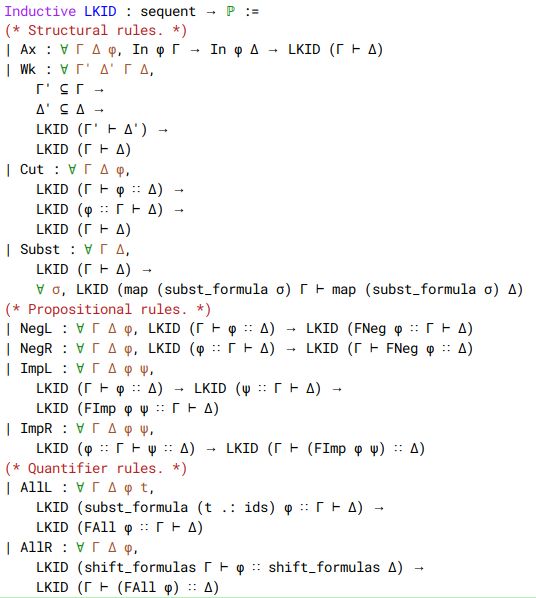
\includegraphics[height=\textheight]{pravila_obicna}
\end{frame}\addtocounter{framenumber}{-1}

\begin{frame}
  \frametitle{Sistem sekvenata: produkcijska pravila}
  \begin{block}{Produkcija}
    \begin{prooftree}
      \AxiomC{\(  Q_{1}\mathbf{u}_{1}  \ldots   Q_{n}\mathbf{u}_{n}  \)}
      \AxiomC{\(  P_{1}\mathbf{v}_{1}  \ldots   P_{m}\mathbf{v}_{m}  \)}
      \BinaryInfC{\(P\mathbf{t}\)}
    \end{prooftree}
  \end{block}

  \begin{block}{Pravilo}
    \begin{scriptsize}
      \begin{prooftree}
        \AxiomC{\( \Gamma \vdash Q_{1} \mathbf{u}_{1}[\sigma], \Delta \quad \ldots \quad \Gamma \vdash Q_{n}\mathbf{u}_{n}[\sigma], \Delta\)}
        \AxiomC{\( \Gamma \vdash P_{1} \mathbf{v}_{1}[\sigma], \Delta \quad \ldots \quad \Gamma \vdash P_{m} \mathbf{v}_{m}[\sigma], \Delta \)}
        \BinaryInfC{\( \Gamma \vdash P \mathbf{t}[\sigma], \Delta \)}
      \end{prooftree}
    \end{scriptsize}
  \end{block}

  \begin{block}{Primjer}
    \begin{minipage}[t]{0.48\linewidth}
      \begin{prooftree}
        \AxiomC{\( \mathit{Odd}(x) \)}
        % \RightLabel{(\texttt{PA\_prod\_E\_succ})}
        \UnaryInfC{\( \mathit{Even}(s(x)) \)}
      \end{prooftree}
    \end{minipage}
    \begin{minipage}[t]{0.48\linewidth}
      \begin{prooftree}
        \AxiomC{\( \Gamma \vdash \mathit{Odd}(x), \Delta \)}
        \UnaryInfC{\( \Gamma \vdash \mathit{Even}(s(x)), \Delta \)}
      \end{prooftree}
    \end{minipage}
  \end{block}
\end{frame}

\begin{frame}[plain]
  \begin{center}
    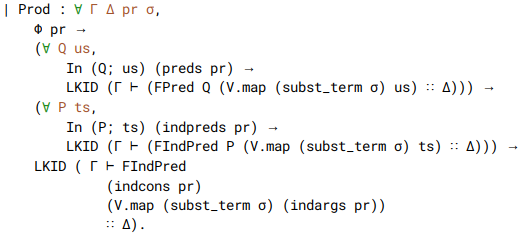
\includegraphics[width=\textwidth]{pravilo_prod}
  \end{center}
\end{frame}\addtocounter{framenumber}{-1}

\begin{frame}[plain]
  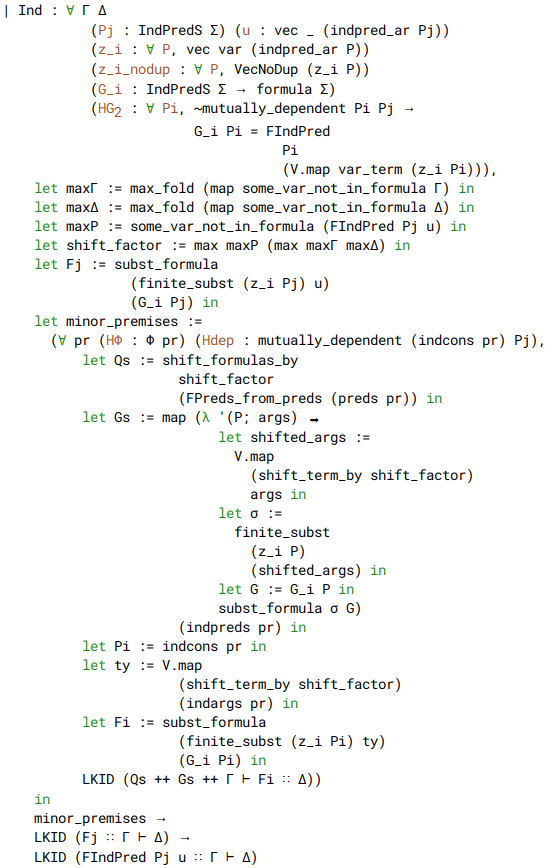
\includegraphics[height=\textheight]{pravilo_ind}
\end{frame}\addtocounter{framenumber}{-1}

\begin{frame}
  \frametitle{Sistem sekvenata: pravila indukcije}
  \begin{block}{Primjer}
    \begin{prooftree}
    \AxiomC{\( \Gamma \vdash G(o), \Delta \)}
    \AxiomC{\( G(x), \Gamma \vdash G(s(x)), \Delta \)}
    \AxiomC{\( G(t), \Gamma \vdash \Delta \)}
    \RightLabel{\( \mathit{(NatInd)} \)}
    \TrinaryInfC{\( \mathit{Nat}(t), \Gamma \vdash \Delta \)}
  \end{prooftree}
\end{block}
\begin{block}{Primjer primjene pravila \textit{NatInd}}
  \begin{scriptsize}
    \begin{prooftree}
      \AxiomC{\(\vdots\)}
      \UnaryInfC{\(\vdash Eo \lor Oo, Ex \lor Ox\)}
      \AxiomC{\(\vdots\)}
      \UnaryInfC{\( Ey \lor Oy \vdash Esy \lor Osy, Ex \lor Ox \)}
      \AxiomC{\(\vdots\)}
      \UnaryInfC{\( Ex \lor Ox \vdash Ex \lor Ox\)}
      \TrinaryInfC{\( Nx \vdash Ex \lor Ox \)}
    \end{prooftree}
  \end{scriptsize}
\end{block}
\end{frame}

\begin{frame}
  \frametitle{Adekvatnost}
  \begin{block}{Teorem}
    Ako je sekventa \textbf{dokaziva} u sustavu \textit{LKID}, \\onda je \textbf{istinita} na standardnim modelima.
  \end{block}
  \begin{alertblock}{Dokaz}
    Indukcijom po strukturi dokaza sekvente \(\Gamma \vdash \Delta\).
  \end{alertblock}
  \begin{itemize}
  \item u disertaciji: šest stranica teksta
  \item u našoj formalizaciji: oko 450 linija
  \end{itemize}
  Problemi kod formalizacije dokaza:
  \begin{itemize}
  \item što je pisac htio reći?
  \item implicitne pretpostavke
  \item implicitno domensko znanje
  \end{itemize}
  
\end{frame}

\begin{frame}
  \frametitle{Zaključak}
  Formalizacija
  \begin{itemize}
  \item sintaksa i semantika logike prvog reda s induktivnim definicijama
  \item dokazni sustav \(\mathit{LKID}\)
  \item oko \textbf{140 lema i dokaza}
  \end{itemize}
  Tekst
  \begin{itemize}
  \item osnovno o Coqu
  \item \textbf{opis formalizacije}
  \item ilustracija cikličkih dokaza
  \end{itemize}
  Što dalje?
  \begin{itemize}
  \item potpunost
  \item dokazni sustav \(\mathit{CLKID}^{\omega}\)
  \item formalno verificirani dokazivač teorema
  \end{itemize}
\end{frame}

\setbeamertemplate{footline}{}
\begin{frame}
  \begin{center}
    \begin{huge}
      Hvala!
    \end{huge}
  \end{center}
\end{frame}\addtocounter{framenumber}{-1}

\begin{frame}
  \frametitle{Hijerarhija tipova u Coqu}
  \begin{scriptsize}
    \begin{forest}
      for tree={l sep+=2mm}
      [\vdots
      [\coqtype{m+1}
      [\ldots]
      [\texttt{bool\(\rightarrow\)\coqtype{m}}]
      [\coqtype{m} [\ldots][\vdots
      [\coqtype{1}
      [\coqset [\texttt{bool}\\ \texttt{nat}\\ \vdots, align=center, base=top] [\texttt{list nat}\\ \texttt{prod nat bool}\\ \texttt{nat\(\rightarrow\)nat}\\ \vdots{}, align=center, base=top] [\ldots]]
      [\texttt{bool}\(\rightarrow\)\coqset]
      [\ldots]
      [\coqprop [\texttt{True}\\ \texttt{1+1=2}\\ \vdots, align=center, base=top] [\texttt{False}\\ \texttt{\(\forall\)b,negb b=b}\\ \vdots, align=center, base=top] [\ldots]]
      [\texttt{nat}\(\rightarrow\)\coqprop]
      [\ldots]
      ]
      ] [\ldots]
      ] [\coqtype{m} \(\rightarrow\) \coqprop] [\ldots]]]
    \end{forest}
  \end{scriptsize}
\end{frame}\addtocounter{framenumber}{-1}

\begin{frame}
  \frametitle{Curry--Howardova korespondencija}
  \begin{center}
    \begin{tabular}[!htb]{rl}
      \toprule
      Dokazivanje & Programiranje \\
      \midrule
      propozicija & tip \\
      dokaz & program \\
      laž & prazan tip \\
      istina & nastanjen tip \\    
      konjunkcija & produktni tip \\
      disjunkcija & zbrojni tip \\
      implikacija & funkcijski tip \\
      univerzalna kvantifikacija & zavisni produkt \\
      egzistencijalna kvantifikacija & zavisna suma \\
      \bottomrule
    \end{tabular}
  \end{center}
\end{frame}\addtocounter{framenumber}{-1}

\begin{frame}
  \frametitle{Ograničenja Coqovog tipskog sustava}
  \begin{itemize}
  \item uvjet pozitivnosti
  \item uvjet strukturalne rekurzije
  \item uvjet produktivnosti
  \item ograničenje na eliminaciju propozicije
  \end{itemize}
\end{frame}\addtocounter{framenumber}{-1}

\begin{frame}[fragile]
  \frametitle{Peanova signatura}
  \begin{scriptsize}
\begin{minted}{coq}
Inductive Func__PA :=
| PA_zero
| PA_succ
| PA_add
| PA_mult.
Definition fun_ar__PA (s : Func__PA) : nat :=
  match s with
  | PA_zero => 0
  | PA_succ => 1
  | PA_add  => 2
  | PA_mult => 2
  end.

Inductive Pred__PA := PA_eq.
Definition pred_ar__PA (s : Pred__PA) : nat := 2.

Inductive IndPred__PA :=
| PA_Nat
| PA_Even
| PA_Odd.
Definition indpred_ar__PA (s : IndPred__PA) : nat := 1.
\end{minted}
  \end{scriptsize}
\end{frame}
\addtocounter{framenumber}{-1}

\begin{frame}[fragile]
  \frametitle{Peanova signatura}
\begin{minted}{coq}
Definition Σ__PA : signature
  := {|
    FuncS := Func__PA;
    fun_ar := fun_ar__PA;
    PredS := Pred__PA;
    pred_ar := pred_ar__PA;
    IndPredS := IndPred__PA;
    indpred_ar := indpred_ar__PA;
  |}.
\end{minted}
\end{frame}
\addtocounter{framenumber}{-1}

\begin{frame}[fragile]
  \frametitle{Primjer skupa produkcija}
  \begin{tiny}
\begin{minted}{coq}
Definition PA_prod_N_zero : production Σ__PA.
  refine (mkProd nil nil PA_Nat _).
  refine [TFunc PA_zero []].
Defined.

Definition PA_prod_N_succ : production Σ__PA.
  refine (mkProd nil _ PA_Nat _).
  - refine (cons _ nil). exists PA_Nat; refine [var_term 0].
  - refine [TFunc PA_succ [var_term 0]].
Defined.

Definition PA_prod_E_zero : production Σ__PA.
  refine (mkProd nil nil PA_Even _).
  refine [ TFunc PA_zero []].
Defined.

Definition PA_prod_E_succ : production Σ__PA.
  refine (mkProd nil _ PA_Even _).
  - refine (cons _ nil). exists PA_Odd; refine [var_term 0].
  - refine [TFunc PA_succ [var_term 0]].
Defined.

Definition PA_prod_O_succ : production Σ__PA.
  refine (mkProd nil _ PA_Odd _).
  - refine (cons _ nil). exists PA_Even; refine [var_term 0].
  - refine [TFunc PA_succ [var_term 0]].
Defined.
\end{minted}
  \end{tiny}
\end{frame}
\addtocounter{framenumber}{-1}

\begin{frame}[fragile]
  \frametitle{Formalizacija standardne Peanove strukture}
  \begin{scriptsize}
\begin{minted}{coq}
Inductive EVEN : nat -> Prop :=
| EO : EVEN 0
| ES : forall n, ODD n -> EVEN (S n)
with ODD : nat -> Prop :=
| OS : forall n, EVEN n -> ODD (S n).

Definition M__PA : structure Σ__PA.
  refine (Build_structure nat _ _ _).
  - intros f; destruct f.
    + intros. exact 0.
    + intros n. exact (S (V.hd n)).
    + intros xy. exact (V.hd xy + V.hd (V.tl xy)).
    + intros xy. exact (V.hd xy * V.hd (V.tl xy)).
  - intros P args; destruct P.
    exact (V.hd args = V.hd (V.tl args)).
  - intros P args; destruct P. 
    + exact (NAT (V.hd args)).
    + exact (EVEN (V.hd args)).
    + exact (ODD (V.hd args)).
Defined.
\end{minted}
  \end{scriptsize}
\end{frame}
\addtocounter{framenumber}{-1}

\begin{frame}[fragile]
  \frametitle{Još jedna korisna lema}
  \begin{tiny}
\begin{minted}{coq}
  Lemma strong_form_subst_sanity2 :
    forall (Σ : signature) (φ : formula Σ) (σ : var -> term Σ)
      (M : structure Σ) (ρ : env M),
      ρ ⊨ (subst_formula σ φ) <-> (σ >> eval ρ) ⊨ φ.
  Proof.
    intros Σ φ; induction φ; intros σ M ρ; cbn; intuition.
    - erewrite <- vec_comp.
      + eauto.
      + intros u; asimpl; now rewrite eval_comp.
    - erewrite vec_comp.
      + eapply H.
      + intros u; asimpl; now rewrite eval_comp.
    - erewrite <- vec_comp.
      + eapply H.
      + intros u; asimpl; now rewrite eval_comp.
    - erewrite vec_comp.
      + eapply H.
      + intros u; asimpl; now rewrite eval_comp.
    - now apply H, IHφ.
    - now apply H, IHφ. 
    - apply IHφ2; apply H; apply IHφ1; auto.
    - apply IHφ2; apply H; apply IHφ1; auto.
    - asimpl in H. specialize H with d.
      apply IHφ in H. asimpl in H. simpl in H.
      rewrite eval_shift in H. apply H.
    - rewrite IHφ. asimpl. simpl.
      rewrite eval_shift.
      apply H.
  Qed.
\end{minted}
  \end{tiny}
\end{frame}
\addtocounter{framenumber}{-1}

\begin{frame}
  \frametitle{Primjer aproksimiranja skupa produkcija}
  Aproksimiramo skup produkcija \(\Phi_{\mathit{PA}}\) na strukturi \(M_{\mathit{PA}}\).\\
  \begin{minipage}{0.19\textwidth}
    \begin{prooftree}
      \AxiomC{}
      \UnaryInfC{\( \mathit{Nat}(o) \)}
    \end{prooftree}
  \end{minipage}
  \begin{minipage}{0.19\textwidth}
    \begin{prooftree}
      \AxiomC{\( \mathit{Nat}(x) \)}
      \UnaryInfC{\( \mathit{Nat}(s(x)) \)}
    \end{prooftree}
  \end{minipage}
  \begin{minipage}{0.19\textwidth}
    \begin{prooftree}
      \AxiomC{}
      \UnaryInfC{\( \mathit{Even}(o) \)}
    \end{prooftree}
  \end{minipage}
  \begin{minipage}{0.19\textwidth}
    \begin{prooftree}
      \AxiomC{\( \mathit{Odd}(x) \)}
      \UnaryInfC{\( \mathit{Even}(s(x)) \)}
    \end{prooftree}
  \end{minipage}
  \begin{minipage}{0.19\textwidth}
    \begin{prooftree}
      \AxiomC{\( \mathit{Even}(x) \)}
      \UnaryInfC{\( \mathit{Odd}(s(x)) \)}
    \end{prooftree}
  \end{minipage}

  \begin{align*}
    (N, E, O)^{0} & = (\varnothing, \varnothing, \varnothing) \\
    (N, E, O)^{1} & = (\{ 0 \}, \{ 0 \}, \varnothing) \\
    (N, E, O)^{2} & = (\{ 0, 1 \}, \{0 \}, \{1\}) \\
    (N, E, O)^{3} & = ( \{0, 1, 2\}, \{0, 2\}, \{1\} ) \\
    (N, E, O)^{4} & = (\{0, 1, 2, 3\}, \{0, 2\}, \{1, 3\}) \\
    (N, E, O)^{5} & = (\{0, 1, 2, 3, 4\}, \{0, 2, 4\}, \{1, 3\}) \\
    (N, E, O)^{6} & = \ldots \\
                  & \vdots \\
    (N, E, O)^{\omega} & = (\mathbb{N}, \mathbb{E}, \mathbb{O})
  \end{align*}
\end{frame}
\addtocounter{framenumber}{-1}

\begin{frame}[fragile]
  \frametitle{Aproksimacije, formalno}
  \begin{footnotesize}
\begin{minted}{coq}
Definition φ_pr
  (pr : production Σ)
  (interp : InterpInd)
  (ds : vec M (indpred_ar (indcons pr)))
  : Prop :=
      exists (ρ : env M),
      (forall Q us, List.In (Q; us) (preds pr) ->
               interpP Q (V.map (eval ρ) us)) /\
        (forall P ts, List.In (P; ts) (indpreds pr) ->
                  interp P (V.map (eval ρ) ts)) /\
        ds = V.map (eval ρ) (indargs pr).
\end{minted}
  \end{footnotesize}
\end{frame}
\addtocounter{framenumber}{-1}

\begin{frame}[fragile]
  \frametitle{Aproksimacije, formalno}
  \begin{scriptsize}
\begin{minted}{coq}
Definition φ_P
  (P : IndPredS Σ)
  (interp : InterpInd)
  : vec M (indpred_ar P) -> Prop.
  refine (fun ds => _).
  refine (@ex (production Σ) (fun pr => _)).
  refine (@ex (P = indcons pr /\ Φ pr) (fun '(conj Heq HΦ) => _)).
  rewrite Heq in ds.
  exact (φ_pr pr interp ds).
Defined.

Definition φ_Φ (interp : InterpInd) : InterpInd :=
  fun P => φ_P P interp.
\end{minted}
  \end{scriptsize}
\end{frame}
\addtocounter{framenumber}{-1}

\begin{frame}[fragile]
  \begin{tiny}
\begin{minted}{coq}
Lemma φ_Φ_ω_least_prefixed : least prefixed φ_Φ_ω.
Proof.
  split.
  - intros P v H.
    unfold φ_Φ, φ_P, φ_pr in H;
      destruct H as (pr & [Heq Hpr] & (ρ & Hpreds & Hindpreds & Heval)). 
    unfold eq_rect in Heval; subst P; subst v.
    enough (Hsup : exists α, forall P ts,
      In (P; ts) (indpreds pr) -> φ_Φ_n α P (V.map (eval ρ) ts)).
    + destruct Hsup as [κ Hsup].
      exists (S κ), pr, (conj eq_refl Hpr), ρ; split; auto.
    + induction (indpreds pr) as [| [P' v'] indpreds' IH].
      * exists 0; inversion 1.
      * pose proof (Hindpreds P' v').
        assert (Hin: In (P'; v') ((P'; v') :: indpreds')) by now left.
        apply H in Hin as [α Hα].
        assert (IH_help : forall P ts,
          In (P; ts) indpreds' -> φ_Φ_ω P (V.map (eval ρ) ts)).
        { intros P ts Hin. apply Hindpreds. now right. }
        apply IH in IH_help as [β Hβ].
        exists (S (max α β)).
        intros P ts Hin; inversion Hin.
        -- apply φ_Φ_n_monotone with α; auto with arith.
           inversion H0; subst P.
           apply inj_pair2 in H0; now subst.
        -- apply φ_Φ_n_monotone with β; auto with arith.
  - intros interp Hprefixed P v Hω.
    destruct Hω as [α Hφ].
    enough (H: forall β, φ_Φ (φ_Φ_n β) P v -> φ_Φ interp P v).
    + now apply Hprefixed, (H α), φ_Φ_n_succ.
    + intros β; apply φ_Φ_monotone. induction β as [| β IH].
      * inversion 1.
      * cbn; unfold prefixed in Hprefixed.
        apply φ_Φ_monotone in IH. red; auto.
Qed.
\end{minted}
  \end{tiny}
\end{frame}
\addtocounter{framenumber}{-1}

\begin{frame}
  \frametitle{Primjer dokaza u sustavu \textit{LKID}}
    \begin{prooftree}
    \AxiomC{}
    \RightLabel{\(\mathit{(Ax)}\)}
    \UnaryInfC{\( \varphi \vdash \varphi\)}
    \RightLabel{\(\mathit{(NegR)}\)}
    \UnaryInfC{\( \vdash \neg\varphi, \varphi\)}
    \RightLabel{\(\mathit{(Perm)}\)}
    \UnaryInfC{\( \vdash \varphi, \neg\varphi\)}
    \RightLabel{\(\mathit{(OrR)}\)}
    \UnaryInfC{\( \vdash \varphi \lor \neg\varphi\)}
  \end{prooftree}
\end{frame}\addtocounter{framenumber}{-1}

\begin{frame}
  \frametitle{Primjer dokaza u sustavu \textit{LKID}}
    \begin{prooftree}
    \AxiomC{}
    \RightLabel{\(\mathit{(Ax)}\)}
    \UnaryInfC{\(\varphi \vdash \varphi, \Delta\)}
    \RightLabel{\(\mathit{(NegL)}\)}
    \UnaryInfC{\(\neg \varphi, \varphi \vdash \Delta\)}
    \RightLabel{\(\mathit{(Perm)}\)}
    \UnaryInfC{\(\varphi, \neg\varphi \vdash \Delta\)}
    \RightLabel{\(\mathit{(AndL)}\)}
    \UnaryInfC{\(\varphi \land \neg \varphi \vdash \Delta\)}
  \end{prooftree}
\end{frame}\addtocounter{framenumber}{-1}

\begin{frame}
  \frametitle{Primjer dokaza u sustavu \textit{LKID}}
    \begin{prooftree}
    \AxiomC{}
    \RightLabel{\( \mathit{(Ax)} \)}
    \UnaryInfC{\( Ex \vdash Ex, Essx \)}
    \RightLabel{\(\mathit{(Prod)} \)}
    \UnaryInfC{\( Ex \vdash Osx, Essx \)}
    \AxiomC{}
    \RightLabel{\( \mathit{(Ax)} \)}
    \UnaryInfC{\( Ex, Osx \vdash Osx \)}
    \RightLabel{\(\mathit{(Prod)} \)}
    \UnaryInfC{\( Ex, Osx \vdash Essx \)}
    \RightLabel{\( \mathit{(Cut)} \)}
    \BinaryInfC{\( Ex \vdash Essx \)}
    \RightLabel{\( \mathit{(ImpR)} \)}
    \UnaryInfC{\(  \vdash Ex \rightarrow Essx \)}
    \RightLabel{\( \mathit{(AllR)} \)}
    \UnaryInfC{\( \vdash \forall x, Ex \rightarrow Essx \)}
  \end{prooftree}
\end{frame}\addtocounter{framenumber}{-1}

\begin{frame}
  \frametitle{Primjer dokaza u sustavu \(\mathit{CLKID}^{\omega}\)}
    \begin{prooftree}
    \AxiomC{}
    \RightLabel{(\textit{Prod})}
    \UnaryInfC{\(\vdash Eo, Oo\)}
    \AxiomC{\(Nx \vdash Ex, Ox \, (\dagger)\)}
    \RightLabel{\( \mathit{(Subst)} \)}
    \UnaryInfC{\(Ny \vdash Ey, Oy\)}
    \RightLabel{\(\mathit{(Perm)}\)}
    \UnaryInfC{\( Ny \vdash Oy, Ey \)}
    \RightLabel{(\textit{Prod})}
    \UnaryInfC{\( Ny \vdash Oy, Osy \)}
    \RightLabel{(\textit{Prod})}
    \UnaryInfC{\(Ny \vdash Esy, Osy\)}
    \RightLabel{\(\mathit{(EqL)}\)}
    \UnaryInfC{\(x = sy, Ny \vdash Ex, Ox\)}
    \RightLabel{\(\mathit{(Case \, N)}\)}    
    \BinaryInfC{\( Nx \vdash Ex, Ox \, (\dagger) \)}
    \RightLabel{\(\mathit{(OrR)}\)}
    \UnaryInfC{\( Nx \vdash Ex \lor Ox \)}
    \RightLabel{\(\mathit{(ImpR)}\)}
    \UnaryInfC{\(\vdash Nx \rightarrow Ex \lor Ox\)}
    \RightLabel{\(\mathit{(AllR)}\)}
    \UnaryInfC{\(\vdash \forall x, Nx \rightarrow Ex \lor Ox\)}
  \end{prooftree}
\end{frame}\addtocounter{framenumber}{-1}

\end{document}
%%% Local Variables:
%%% mode: LaTeX
%%% TeX-master: t
%%% End:
